\documentclass{article}

\usepackage{graphicx}

\title{Learning MC algorithms}
\author{Lee Hwee Kuan}

\begin{document}
\maketitle

Consider a system of 2D Ising spins $\sigma = (s_1,s_2, \cdots s_n)$ with $s_i =\pm 1$
on a squre lattice of size $L \times L$ sites.
Hamiltonian is 
\begin{equation}
E(\sigma) = - \sum_{\langle i,j\rangle} s_i s_j
\end{equation}
where $\langle i,j \rangle$ represents summation over nearest neighbors on 
the square lattice. Each edge on this graph is sum over once.
The objective is to make a RevNet that learns how to do MCMC with detailed balance
condition satisfied.

\section{Implementation in tensorflow and matrix representation of Hamilitonian}

Tensorflow works with linear algebra and hence we need to express our equations
in matrix formulation. Let $\Sigma$ be the 2D spin configurations in the form
of a matrix, elements in the matrix corresponds to the site in the square lattice.
\begin{equation}
E = \frac{1}{L^2} \left(
\|\Sigma * \left( \Sigma \cdot S^l \right)\| +\| \Sigma * \left( S^u \cdot \Sigma \right)\|
\right)
\label{eq:E}
\end{equation}
where $S^l$ and $S^u$ are matrices that rotate the columns and rows matrix elements such that 
when the resultant matrix multiply by the original spin matrix $\Sigma$ element wise $*$, 
then sum element wise gives the hamiltonian. $\|\cdot\|$ represents summing over elements
in a matrix.
\begin{equation}
S^u = \left( \begin{array}{cccccc}
0  &-1 & 0 & \cdots & 0 & 0 \\
0  & 0 &-1 & \cdots & 0 & 0 \\
\vdots & & & & \\
0  & 0 & 0 & \cdots &-1 & 0 \\
0  & 0 & 0 & \cdots & 0 &-1 \\
-1 & 0 & 0 & \cdots & 0 & 0 \\
\end{array} \right)
\end{equation}
\begin{equation}
S^l = \left( \begin{array}{cccccc}
0   & 0 & 0 & \cdots & 0 & -1 \\
-1  & 0 & 0 & \cdots & 0 & 0 \\
0   &-1 & 0 & \cdots & 0 & 0 \\
\vdots & & & & \\
0  & 0 & 0 & \cdots & 0 & 0 \\
0  & 0 & 0 & \cdots &-1 & 0 \\
\end{array} \right)
\end{equation}

\subsection{Tensorflow batch handling}
The implementation in tensorflow handles data in batch. We rewrite 
Eq.(\ref{eq:E}) in terms
of batch and matrix indexing, Eq.(\ref{eq:E}) becomes,
\begin{eqnarray} \nonumber
E^b & = & \frac{1}{L^2} \left( 
             \sum_{i,j,k} \Sigma^b_{ij} \Sigma^b_{ik} S^l_{kj} +
             \sum_{i,j,k} \Sigma^b_{ij} S^u_{jk} \Sigma^b_{ki} 
          \right) \\
    & = & \frac{1}{L^2} \sum_{i,j,k} \Sigma^b_{ij}\left( 
              \Sigma^b_{ik} S^l_{kj} + S^u_{jk} \Sigma^b_{ki} 
          \right) 
\end{eqnarray}
$b$ is the index for individual data in the batch. $\Sigma^b$ is the $b$th
spin configuration.

\section{RevNet architecture}
RevNet is originally proposed by A.N.Gomez {\it et al} (arXiv:1707.04585v1).
It is a network that is reversible, that is the network has a dual network
which flips the input and output exactly. The network takes two inputs and
generate two outputs, its dual takes in the outputs generated by the original 
network and generates the inputs of the original network.
The ising spin magnitude is $\pm 1$ and therefore the RevNet has to be
modified a little to satisfy this constraint. Fig. \ref{fig:revnet} shows 
the network architecture applicable for the Ising model.
%
%\begin{figure}
%\center{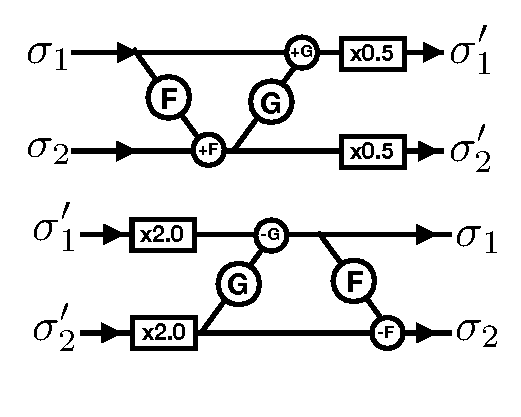
\includegraphics[width=8cm]{./revnet.pdf}}
%\caption{Figure illustrates RevNet with inputs $\sigma_1,\sigma_2$ to generate
%outputs $\sigma'_1,\sigma'_2$. Its dual shown in the lower figure takes 
%in $\sigma'_1,\sigma'_2$
%and outputs $\sigma_1,\sigma_2$. 
%$F$ and $G$ can be any neural network or any 
%transformation functions.}
%\label{fig:revnet}
%\end{figure}
%
Equations for RevNet are,
\begin{eqnarray} 
\sigma'_2 & = & \frac{1}{2}[ \sigma_2 + F(\sigma_1) ] \\ \nonumber
\sigma'_1 & = & \frac{1}{2}[ \sigma_1 + G(\sigma'_2) ] \\ \nonumber
\sigma_1 & = & 2 \sigma'_1 - F(\sigma'_2) \\ \nonumber
\sigma_2 & = & 2 \sigma'_2 - G(\sigma_1) 
\end{eqnarray}
$F$ and $G$ can be any network or transformation. In our implementation
we use the hyperbolic tangent activation function, the reason being than
hyperbolic tangent function is bounded by $\pm 1$. 

\section{Using RevNet to recover detailed balance}
Detailed balance can be recovered by replacing MLP with RevNet. 
RevNet takes in two spin configurations, $\sigma_1,\sigma_2$
and output two configurations $\sigma_1',\sigma_2'$.
In RevNet, there are two ends of the network, feed data into
one end and the output will be on the other end and vice versa.
For clarity, we define the directions ``forward" and ``backward"
but since RevNet is symmetric, forward and backward definition
is arbitrarily fixed.
Algorithm goest like this
\begin{enumerate}
\item Given configurations $\sigma_1,\sigma_2$
\item Pass $\sigma_1,\sigma_2$ through RevNet in the forward 
or backward direction with the same probability
to generate $\sigma_1',\sigma_2'$
\item Accept the new configurations $\sigma_1',\sigma_2'$ with the probability
\begin{equation}
A(\sigma_1,\sigma_2 \rightarrow \sigma_1',\sigma_2') = \min(1,\exp(-\beta [(E_1'-E_1)+(E_2'-E_2)] ))
\end{equation}
\end{enumerate}
When the RevNet learns the transitions with $(E_1+E_2)\approx (E_1'+E_2')$, 
this algorithm becomes efficient.

\subsection{Proof of detailed balance condition}
Proof of detailed balance condition of the above algorithm is as follows.
Assuming configurations $\sigma_1,\sigma_2$ are sampled independently
from the equilibrium distribution then the probability of sampling is
\begin{eqnarray} \nonumber
p(\sigma_1,\sigma_2) & = & \exp(-\beta E(\sigma_1)) \exp(-\beta E(\sigma_2))  / {\cal Z}^2 \\
                     & = & \exp(-\beta (E_1+E_2)) / {\cal Z}^2
\end{eqnarray}
Make use of the reversibility of RevNet, the forward and backward 
trial moves probabilities 
between two sets of configurations linked by RevNet are the same, i.e.
\begin{equation}
T[ (\sigma_1 ,\sigma_2 ) \rightarrow (\sigma_1',\sigma_2')] =
T[ (\sigma_1',\sigma_2') \rightarrow (\sigma_1 ,\sigma_2 )] = 0.5
\end{equation}
Then the transition matrix becomes the acceptance matrix
\begin{equation}
\frac{A[ (\sigma_1 ,\sigma_2 ) \rightarrow (\sigma_1',\sigma_2')]}
     {A[ (\sigma_1',\sigma_2') \rightarrow (\sigma_1 ,\sigma_2 )]} = 
     \frac{\exp(-\beta (E_1'+E_2')}
          {\exp(-\beta (E_1 +E_2 )} =
     \frac{p(\sigma_1',\sigma_2')}{p(\sigma_1,\sigma_2)}
\end{equation}

\section{Training the RevNet - the loss function}
The loss function is define on a batch of spin configurations,
\begin{equation}
Loss = \sum_b [(E^b_{1}+E^b_{2}) - ({E'}^b_{1}+{E'}^b_{2})]^2 + 
      \frac{\lambda}{2 L^2} \left[ \| {\Sigma'}^b_1 *{\Sigma'}^b_1 \| +
                     \| {\Sigma'}^b_2 *{\Sigma'}^b_2 \| \right]
\mbox{ with }\lambda<0
\end{equation}
Since the RevNet does not output $s_i = \pm 1$, the second term in the above
equation penalize outputs that gives $\sigma'<1$.
Set activation function to be $tanh$ to bound spins to $\pm 1$.
$L^2$ is the number of lattice sites. It is use to normalize the loss to make it
lattice size invariant.



\end{document}

